\begin{figure}[ht!]
    \centering
    % \begin{tabular}[c]{ccc}
    % \begin{subfigure}[c]{0.31\textwidth}
    %     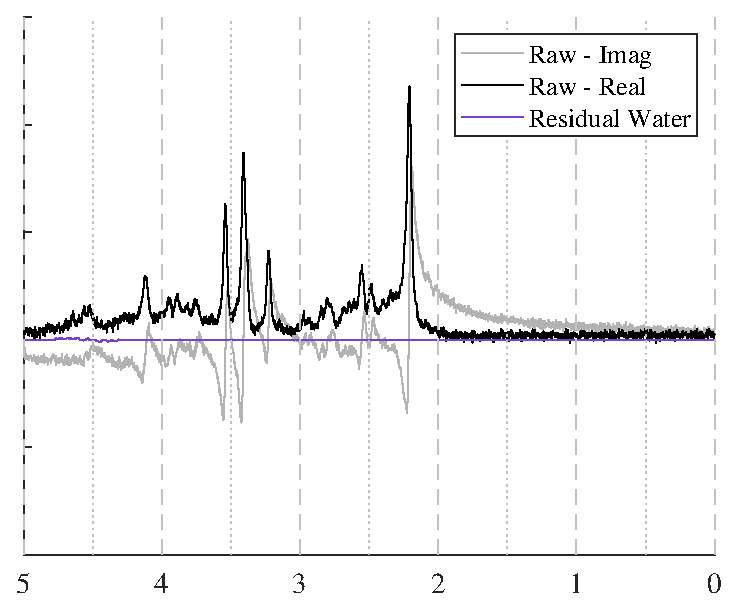
\includegraphics[width=0.93\textwidth]{images/samples_by_artifact/30ms_artifact_samples_fshift_1.eps}
    %     \caption{F\textsubscript{shift} = 0.2 ppm = 160 Hz}
    %     \vspace{3pt}
    % \end{subfigure}&
    % \begin{subfigure}[c]{0.31\textwidth}
    %     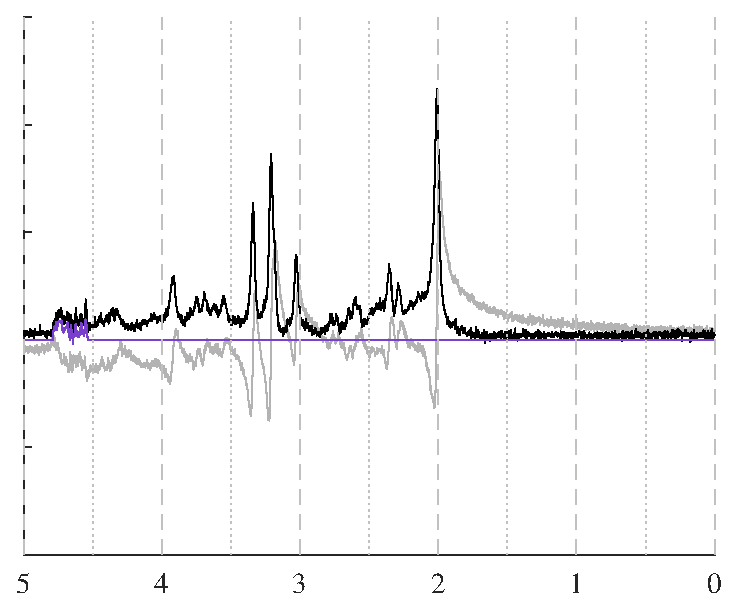
\includegraphics[width=0.93\textwidth]{images/samples_by_artifact/30ms_artifact_samples_fshift_2.eps}
    %     \caption{F\textsubscript{shift} = 0.0 ppm = 0 Hz}
    %     \vspace{3pt}
    % \end{subfigure}&
    % \begin{subfigure}[c]{0.31\textwidth}
    %     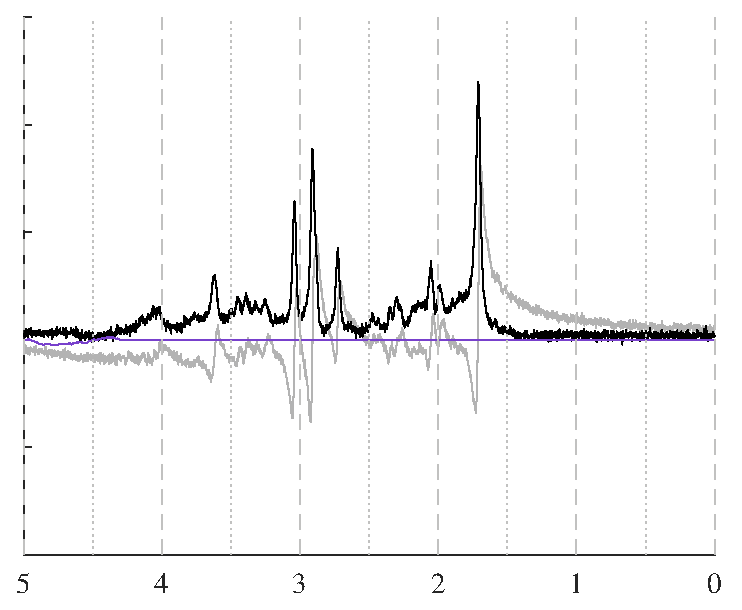
\includegraphics[width=0.93\textwidth]{images/samples_by_artifact/30ms_artifact_samples_fshift_3.eps}
    %     \caption{F\textsubscript{shift} = -0.3 ppm = -240 Hz}
    %     \vspace{3pt}
    % \end{subfigure}\\
    % \begin{subfigure}[c]{0.31\textwidth}
    %     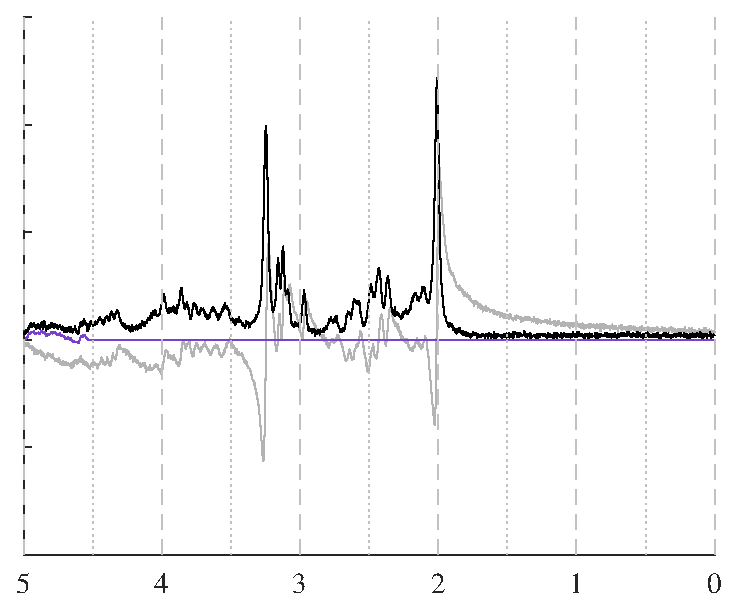
\includegraphics[width=0.93\textwidth]{images/samples_by_artifact/30ms_artifact_samples_fshift_4.eps}
    %     \caption{F\textsubscript{shift} $\in [-0.10, 0.10]$ ppm = $\pm 80$Hz}
    %     \vspace{3pt}
    % \end{subfigure}&
    % \begin{subfigure}[c]{0.31\textwidth}
    %     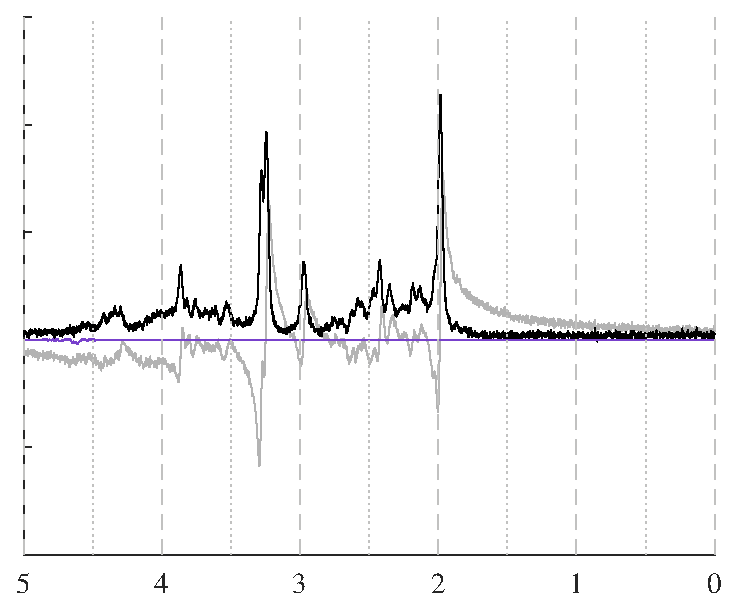
\includegraphics[width=0.93\textwidth]{images/samples_by_artifact/30ms_artifact_samples_fshift_5.eps}
    %     \caption{F\textsubscript{shift} $\in [-0.10, 0.10]$ ppm = $\pm 80$Hz}
    %     \vspace{3pt}
    % \end{subfigure}&%
    % \begin{subfigure}[c]{0.31\textwidth}
    %     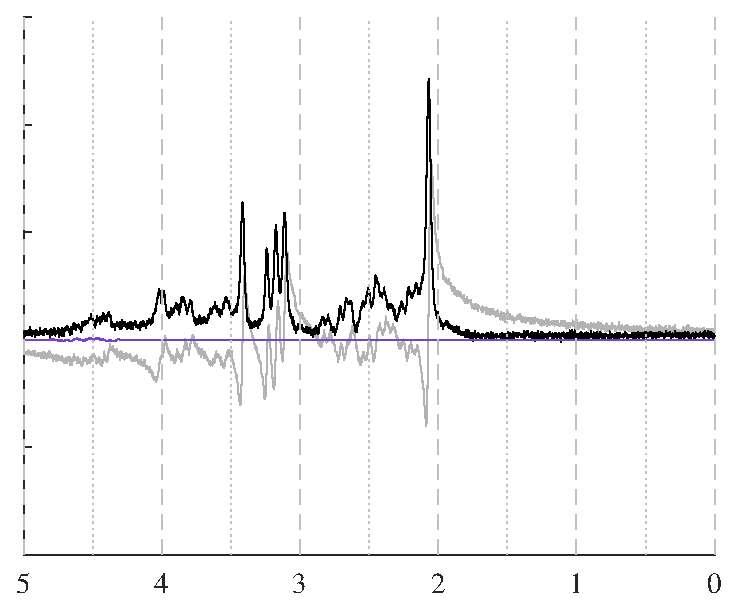
\includegraphics[width=0.93\textwidth]{images/samples_by_artifact/30ms_artifact_samples_fshift_6.eps}
    %     \caption{F\textsubscript{shift} $\in [-0.10, 0.10]$ ppm = $\pm 80$Hz}
    %     \vspace{3pt}
    % \end{subfigure}\\
    % \end{tabular}
    \includegraphics[width=\textwidth,keepaspectratio]{images/compiled_figures/MRS_Sim_Figure_11_Frequency_Shifts_samples.png}
    \caption{Two types of frequency shifts are shown in these examples. The top row shows global frequency shifts. The bottom row shows the effects of using randomly sampled metabolite-level frequency shifts. The spectral SNR = 15 with fixed lorentzian and gaussian broadening. No baselines, phase offsets, or eddy currents were included.}
    \label{fig:30ms samples fshift}
\end{figure}

